\chapter{Einleitung}

\gls{mrt} ist nicht nur in der Humanmedizin, sondern auch in der Kleintierbildgebung eine wichtige Modalität.

 Hinsichtlich der Abbildung von Gewebe ist es anderen bildgebenden Verfahren, wie der \gls{ct}, überlegen: Statt mit Röntgenstrahlung, wie beim \gls{ct}, entstehen die Schnittbilder beim \gls{mrt}-Tomographen durch Ausnutzung des \gls{nmr}-Effekts der Wasserstoffkerne im Körper, welcher einen hohen Weichteilkontrast ermöglicht. Eine \gls{mrt}-Untersuchung verursacht keine Belastung mit ionisierenden Strahlen.
 
\section{Aufgabenstellung}
\tikzstyle{every node}=[yshift=4pt]
%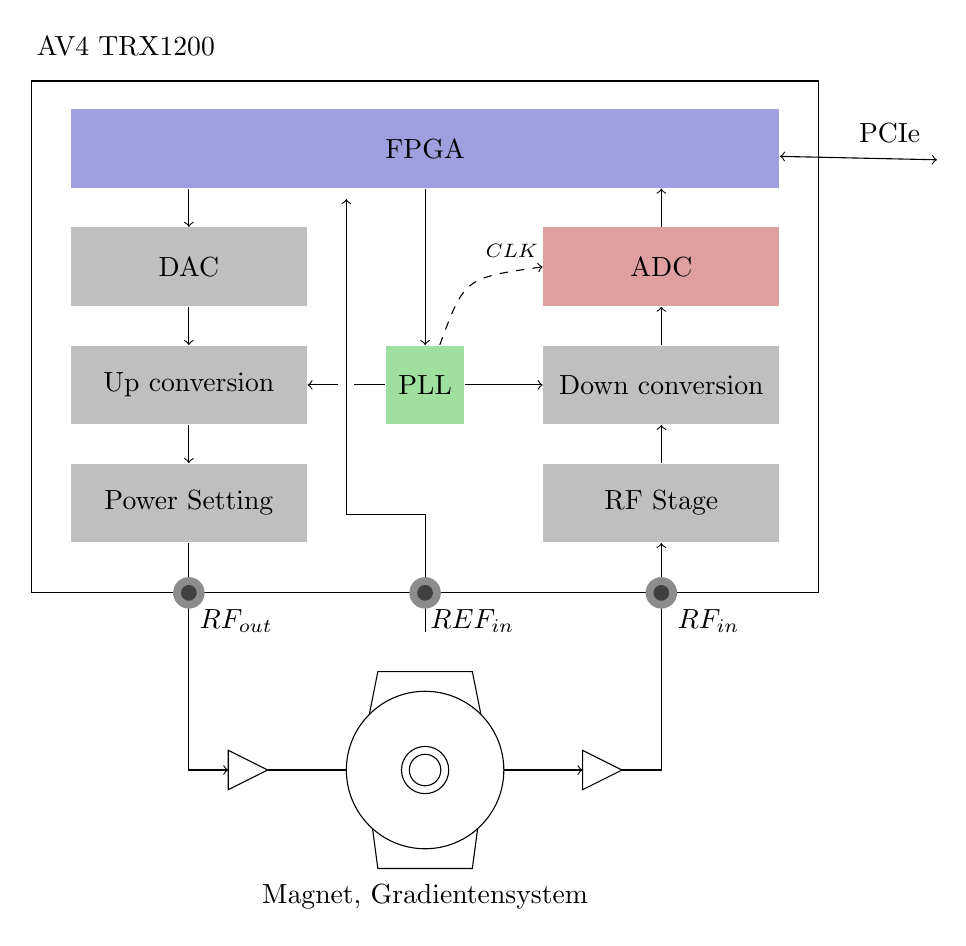
\begin{tikzpicture}[scale=1]
\draw[draw=black] (0,0) rectangle (10,6.5);
\node[fill=gray!50,minimum height=1cm,minimum width=3cm] (DAC) at (2,4) {DAC};
\node[fill=gray!50!red!50,minimum height=1cm,minimum width=3cm] (ADC) at (8,4) {ADC};
\node[fill=gray!50,minimum height=1cm,minimum width=3cm] (UPC) at (2,2.5) {Up conversion};
\node[fill=gray!50,minimum height=1cm,minimum width=3cm] (DWC) at (8,2.5) {Down conversion};
\node[fill=gray!50,minimum height=1cm,minimum width=3cm] (PS) at (2,1) {Power Setting};
\node[fill=gray!50,minimum height=1cm,minimum width=3cm] (RF) at (8,1) {RF Stage};
\node[fill=gray!50!blue!50,minimum height=1cm,minimum width=9cm] (FPGA) at (5,5.5) {FPGA};
\node[fill=gray!50!green!50,minimum height=1cm,minimum width=1cm] (PLL) at (5,2.5) {PLL};

\draw[<-] (PS.north) -- (UPC.south);
\draw[<-] (UPC.north) -- (DAC.south);
\draw[<-] (DAC.north) -- (FPGA.south -| DAC);

\draw[->] (RF.north) -- (DWC.south);
\draw[->] (DWC.north) -- (ADC.south);
\draw[->] (ADC.north) -- (FPGA.south -| ADC);

\draw[->] (PLL) -- (DWC);
\draw[->] (PLL) -- (UPC);
\draw[->] (FPGA) -- (PLL);
\draw[color=white,line width=2mm] (4,2) -- (4,3);
\draw[->] (5,-0.5) |- (4,1) -- (4,5);
\draw[<-] (2.5,-2.25) -| (2,-1) -- (PS);
\draw[->] (7.5,-2.25) -|(8,-1) -- (RF);

\fill[fill=gray!90] (2,0) circle (0.2);\fill[fill=darkgray] (2,0) circle (0.1);
\fill[fill=gray!90] (8,0) circle (0.2);\fill[fill=darkgray] (8,0) circle (0.1);
\fill[fill=gray!90] (5,0) circle (0.2);\fill[fill=darkgray] (5,0) circle (0.1);

\node(REFin) at (5.6,-0.5) {$REF_{in}$};
\node(RFout) at (2.6,-0.5) {$RF_{out}$};
\node(RFin) at (8.6,-0.5) {$RF_{in}$};

\draw (2.5,-2) -- (2.5,-2.5) -- (3,-2.25) -- cycle;
\draw (7,-2) -- (7,-2.5) -- (7.5,-2.25) -- cycle;
\draw[->] (3,-2.25) -- (7,-2.25);

\filldraw[fill=white] (4.4,-3.5) -- (5.6,-3.5) -- (5.8,-2) -- (4.2,-2) -- cycle;
\filldraw[fill=white] (4.4,-1) -- (5.6,-1) -- (5.8,-2) -- (4.2,-2) -- cycle;
\filldraw[fill=white] (5,-2.25) circle(1);
\filldraw[fill=white] (5,-2.25) circle(0.3);
\filldraw[fill=white] (5,-2.25) circle(0.2);

\node(TRX) at (1.2,6.8) {AV4 TRX1200};
\node[text width=6cm,align=center](MAGNET) at (5,-4) {Magnet, Gradientensystem};

\draw[<->] (FPGA) -- (11.5,5.5);
\node[] (PCIe) at (10.9,5.7) {PCIe};

\draw[->,dashed] (PLL) .. controls (5.5,4) .. (ADC.west);
\node[] (clk) at (6.1,4.2) {\scriptsize$CLK$};
\end{tikzpicture}


\todoin[]{Soll/Ist und Anforderungen an die Simulation}